\documentclass[xcolor=dvipsnames]{beamer}

\usepackage[utf8]{inputenc}
\usepackage[french]{babel}
\usepackage[T1]{fontenc}
\usepackage{ulem}
\usepackage{tabularx}
\usepackage{multirow}
\usepackage{xstring}
\usepackage{pifont}

%%% MACRO %%%


% FIXME Prendre en compte les majuscule déjà présente
\makeatletter
\@ifpackageloaded{xstring}{
	\newcommand\smallcaps[1]{\StrLeft{#1}{1}\scriptsize\uppercase{\StrGobbleLeft{#1}{1}}\normalsize }
}{
	\newcommand\smallcaps[1]{\textsc{#1}}
}
\makeatother



%===============================================================================
% Définit un type de puce pour une liste. Si le pakage "pifont" est chargé, il 
% est utilisé, sinon on met un tiret.
\makeatletter
\@ifpackageloaded{pifont}{
	\newcommand\goodItemArrow[0]{\ding{226}}
}{
	\newcommand\goodItemArrow[0]{-}
}
\makeatother



%===============================================================================
% Item de liste avec spécification de la puce et paramètre écrit en gras.
\newcommand\functionality[1]{
	\item[\goodItemArrow] \textbf{#1}\\
}



%===============================================================================
% Commande \Euro indépendante des paquets chargés 
\makeatletter
\@ifpackageloaded{eurosym}{
	\newcommand\Euro[0]{\euro{}}
}{
	\@ifpackageloaded{textcomp}{
		\newcommand\Euro[0]{\texteuro}
	}{
		\newcommand\Euro[0]{Euro}
	}
}
\makeatother



%===============================================================================
% Accès à des variables dans le document. 
%\makeatletter
%\let\titleName\@title
%\let\subtitleName\@subtitle
%\let\authorName\@author
%\makeatother



% Titre de la section courante (que dans beamer)
%\secname 
% Titre de la sous-section courante (que dans beamer)
%\subsecname





\title[Final presentation]{Discrete 3D surfaces of revolution}
\subtitle{Final presentation}
\author[Discret group]{Zied \smallcaps{Ben} \smallcaps{Othmane} \\
	Thomas \smallcaps{Benoist} \\
	Adrien \smallcaps{Bisutti} \\
	Lydie \smallcaps{Richaume}
}
\institute{University of Poitiers}
\date{March 21\textsuperscript{st}, 2016}

\usetheme{Madrid}
\usecolortheme{sidebartab}
\usefonttheme{professionalfonts}

\definecolor{fondtitre}{rgb}{0.0,0.35,0.7}
\setbeamercolor{palette primary}{bg=fondtitre}
\setbeamercolor{palette secondary}{bg=fondtitre!75!black}
\setbeamercolor{palette tertiary}{bg=fondtitre!55!black}
\setbeamercolor{palette quaternary}{bg=fondtitre!35!black}
\setbeamercolor{item}{fg=fondtitre}
\setbeamercolor{block title}{fg=white, bg=fondtitre!85!black}



%%%%%%%%%%%%%%%%%%%%%%%%%%%%%%%%%%%%%%%%%%%%%%%%%%%%%%%%%%%%%%%%%%%%%%%%%%%%%%%%
%	MACRO
%%%%%%%%%%%%%%%%%%%%%%%%%%%%%%%%%%%%%%%%%%%%%%%%%%%%%%%%%%%%%%%%%%%%%%%%%%%%%%%%


% Affichage du plan à chaque début de section
\AtBeginSection[]{
	\setbeamertemplate{background canvas}{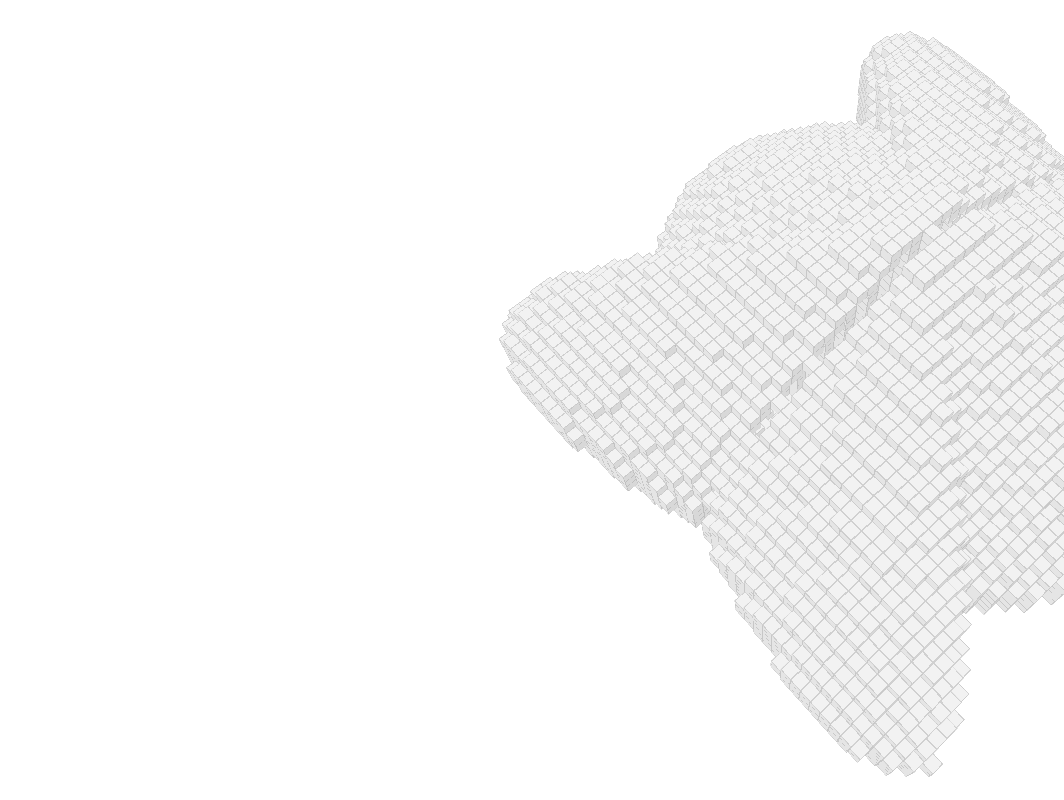
\includegraphics[height=\paperheight, width=\paperwidth]{Images/papillon.png}}
	\begin{frame}{Outline}
	  	\tableofcontents[currentsection, hideothersubsections]
	\end{frame}
	\setbeamertemplate{background canvas}[default]
}


% Nouvelle boîte pour le titre
\newenvironment<>{titleblock}[1]{%
	\setbeamercolor{block body}{fg=white, bg=fondtitre}%
	\begin{block}#2{#1}}{\end{block}}


% Vide la barre de navigation
\setbeamertemplate{navigation symbols}{}



%%%%%%%%%%%%%%%%%%%%%%%%%%%%%%%%%%%%%%%%%%%%%%%%%%%%%%%%%%%%%%%%%%%%%%%%%%%%%%%%
%	DOCUMENT
%%%%%%%%%%%%%%%%%%%%%%%%%%%%%%%%%%%%%%%%%%%%%%%%%%%%%%%%%%%%%%%%%%%%%%%%%%%%%%%%


\begin{document}


%===============================================================================
%	TITRE
%===============================================================================

\begin{frame}
	\titlepage
	
\includegraphics[width=2cm]{../Images/logo-Xlim.png}
	\hfill
	
\includegraphics[width=2cm]{../Images/logo_univ_poitiers.png}
\end{frame}


%===============================================================================
%	PLAN
%===============================================================================


\setbeamertemplate{background canvas}{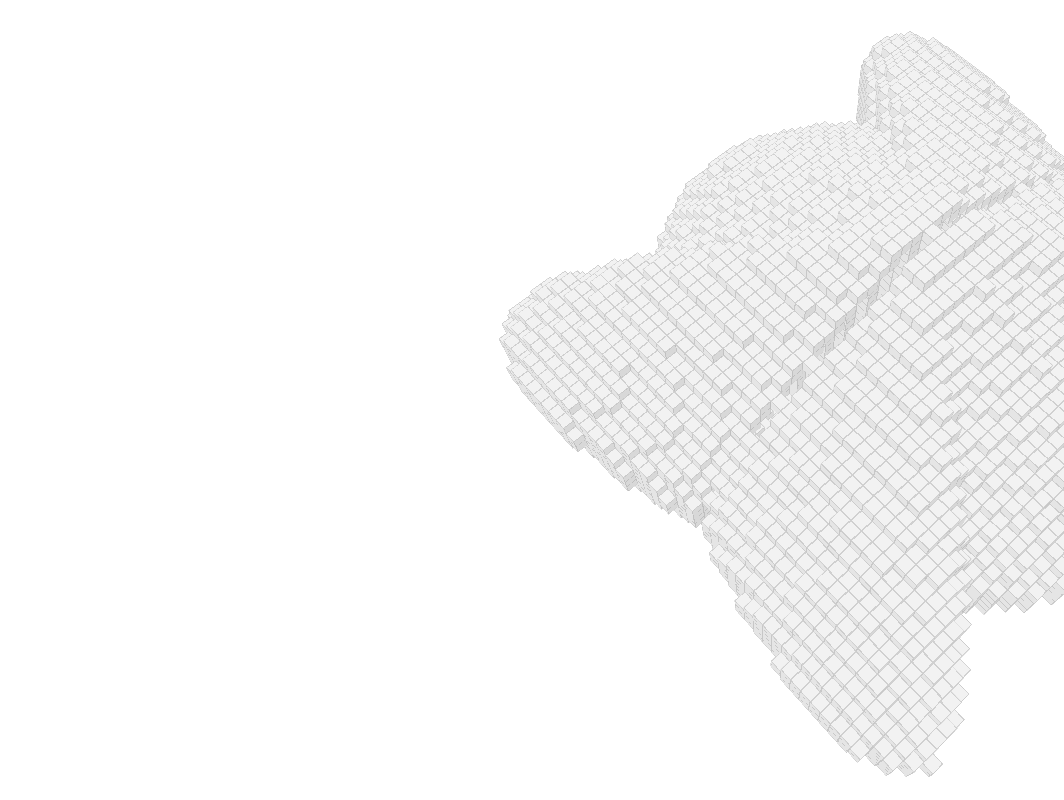
\includegraphics[height=\paperheight, width=\paperwidth]{Images/papillon.png}}
\begin{frame}{Outline}
  	\tableofcontents[hideallsubsections]
\end{frame}
\setbeamertemplate{background canvas}[default]



%===============================================================================
%	INTRODUCTION
%===============================================================================


\section{Introduction}


% --- Équipe -------------------------------------------------------------------
\subsection{Collaborators and clients}
	\begin{frame}{\subsecname}
		\begin{itemize}
			\item Clients:
				\begin{itemize}
					\item \'Eric \smallcaps{Andres} (Professor and former director of 
						\smallcaps{XLIM}-\smallcaps{SIC} department)
					\item Ga\"elle \smallcaps{Largeteau}-\smallcaps{Skapin} (University lecturer, Discrete geometry)
				\end{itemize}
		\end{itemize}
		\begin{itemize}
			\item Exemple of final user:
				\begin{itemize}
					\item Aur\'elie \smallcaps{Mourier} (Artist)
				\end{itemize}
		\end{itemize}
		\begin{itemize}
			\item Pedagogic Supervisor: 
				\begin{itemize}
					\item Philippe \smallcaps{Meseure} (Professor, Computer Graphics)
				\end{itemize}
		\end{itemize}
	\end{frame}


% --- Contexte -----------------------------------------------------------------
\subsection{Context}
	\begin{frame}{\subsecname}
		\begin{itemize}
			\item \'Eric \smallcaps{Andres} and Ga\"elle \smallcaps{Largeteau}-\smallcaps{Skapin}
				developed a new algorithm to model discrete surfaces of revolution.
		\end{itemize}
		
		\begin{figure}
			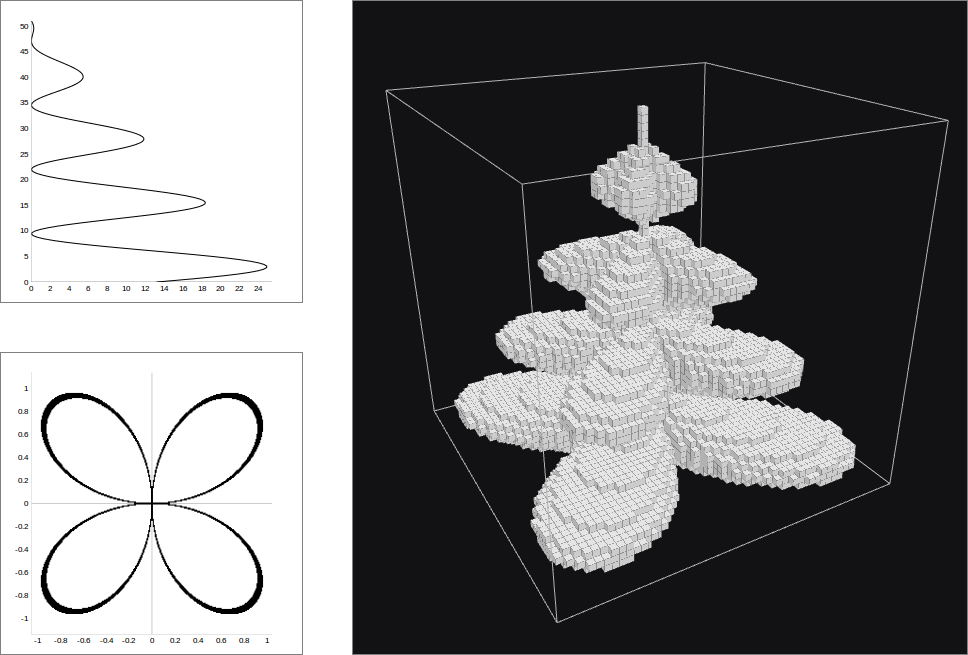
\includegraphics[height=4.7cm]{Images/context.png}
		\end{figure}
	
		\begin{itemize}
			\item Display the result with Mathematica
			\item Need a tool usable by everyone and everywhere
		\end{itemize}
	\end{frame}
	

% --- Objectives ---------------------------------------------------------------
\subsection{Objectives}
	\begin{frame}{\subsecname}
		\begin{itemize}
			\item Surfaces visualization tool
			\begin{itemize}
				\item 3D, slices visualization
				\item Choose the generatrix and directrix
		 		\item Export the results
			\end{itemize}
		\end{itemize}
		\begin{itemize}
			\item Algorithm to generate surfaces of revolution
			\begin{itemize}
				\item Provided by the clients
				\item Possible evolution of the algorithm
			\end{itemize}
		\end{itemize}
	\end{frame}



%===============================================================================
%	TRAVAIL RÉALISÉ
%===============================================================================



\section{Work achieved}

% --- Technological choices -----------------------------------------------------
\subsection{Technological choices}
	\begin{frame}{\subsecname}
	Tool usable by everyone and everywhere $\to$ web application
	\vspace{0.5cm}
		\begin{itemize}
			\item Mathematica?
			\begin{itemize}
				\item Algorithm already implemented for Mathematica
				\item Server application: difficult to set up a server from the university
				\item Client application: user would have to install Mathematica (not free)
			\end{itemize}
			\item Without Mathematica
			\begin{itemize}
				\item Server application: security problems, data transfert
				\item Client application: large quantity of computations $\to$ slow for computers with low capacities
			\end{itemize}
			\item Choice: client application $\to$ {\small{}HTML5/CSS}, Javascript, WebGL
		\end{itemize}
	\end{frame}
	
	
% --- Rappel et persective -----------------------------------------------------
\subsection{Prototype}
	\begin{frame}{\subsecname}
		\begin{figure}
			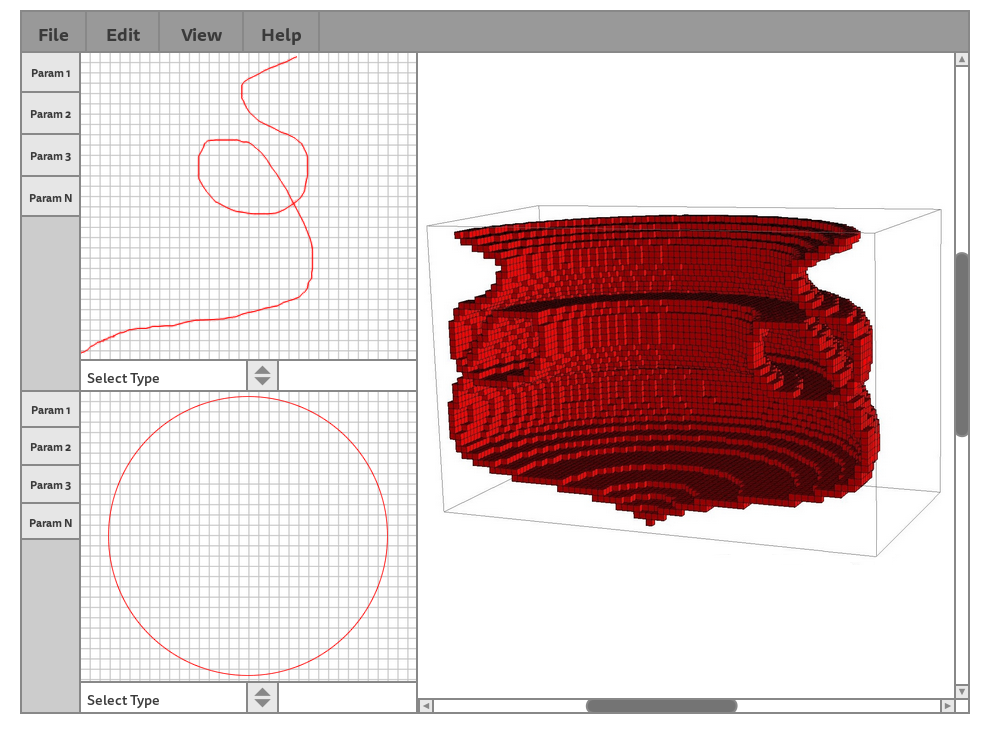
\includegraphics[height=7.8cm]{Images/maquette.png}
		\end{figure}
	\end{frame}


% --- Démonstration ------------------------------------------------------------
\setbeamertemplate{background canvas}{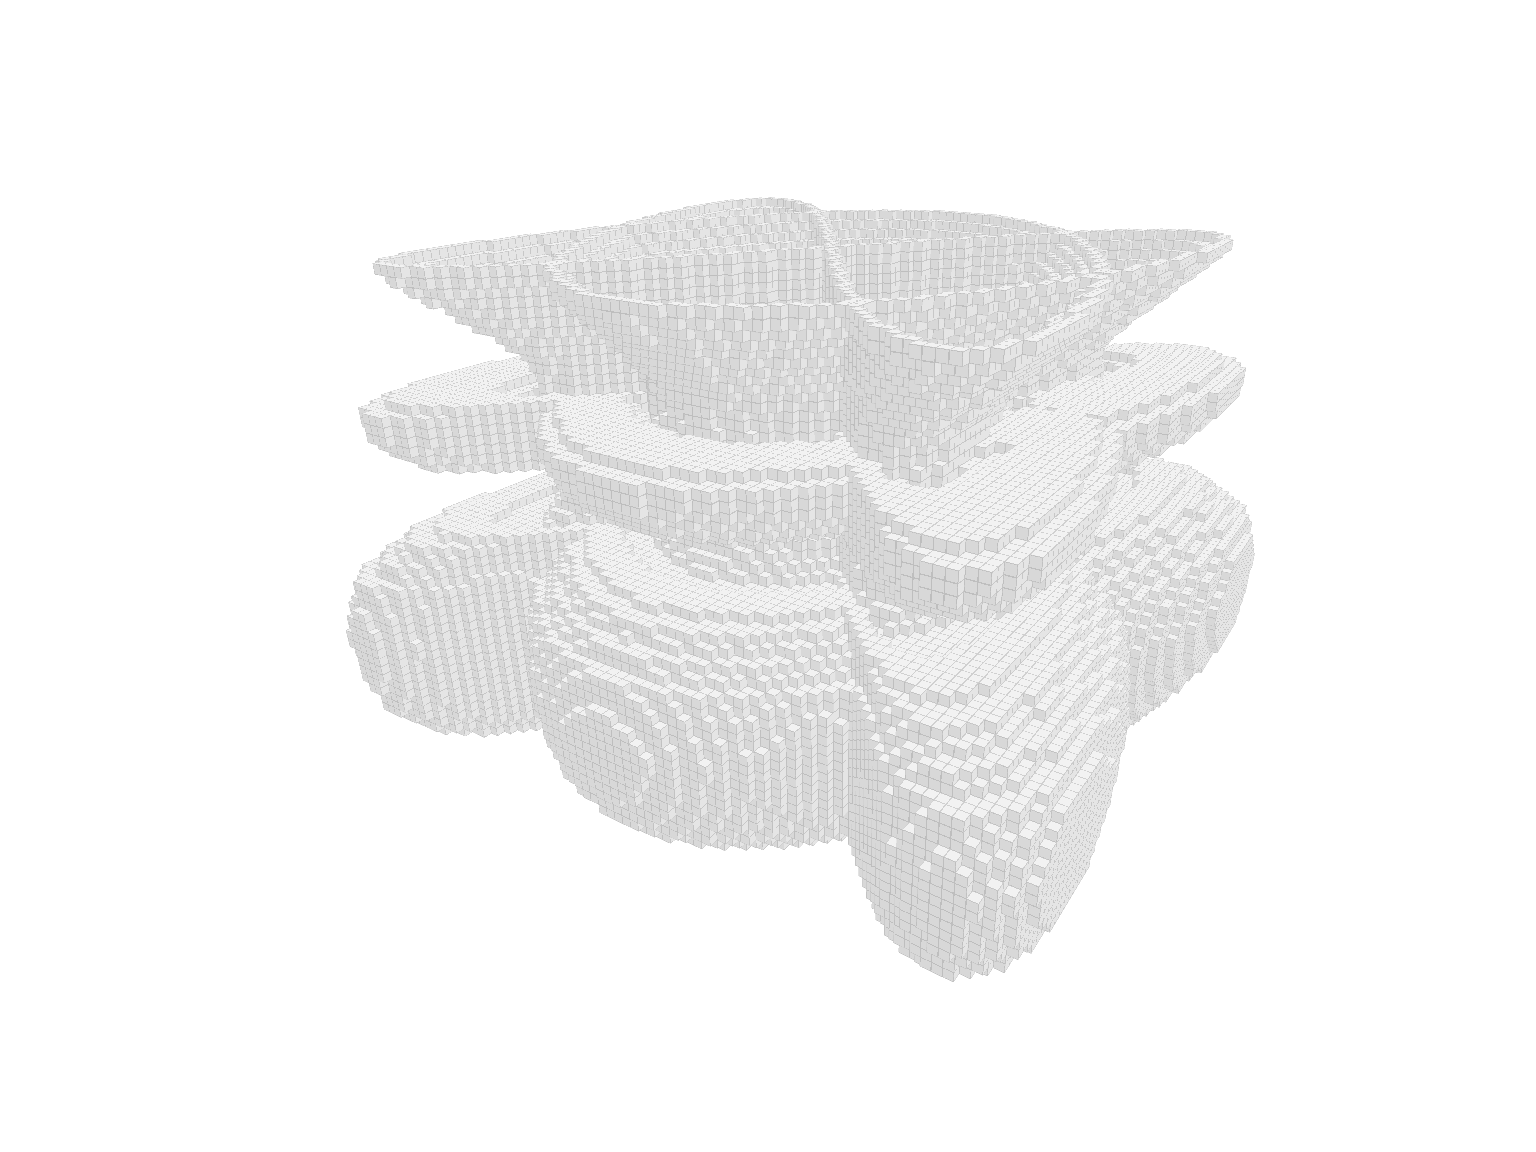
\includegraphics[height=\paperheight, width=\paperwidth]{Images/surface3d2.png}}
\subsection{Demonstration}
	\begin{frame}{\subsecname}
		\begin{center}
			\href
			{run:../../../ApplicationDiscret/Application/discreteSurface.html}
			{\subsecname}
		\end{center}
	\end{frame}

\setbeamertemplate{background canvas}[default]


% --- Aspect technique ---------------------------------------------------------
	\subsection{Technical aspect} 
	\begin{frame}{\subsecname\ - 2D part}
		\begin{itemize}
			\item Curves
			\begin{itemize}
				\item Use MathJS
				\item Two kind of definition: formula or freehand drawing
				\item Formula: parse string $\to$ equation
				\item Freehand drawing: retrieve points from {\small{}HTML5} canvas
			\end{itemize}
		\end{itemize}
		\begin{itemize}
			\item Display
			\begin{itemize}
				\item Explicit curve: easy to display
				\item How to display implicit curves ?
				\item Use functionPlot and {\small{}HTML5} canvas
				\item Formula curves: functionPlot $\to$ {\small{}SVG}
				\item Freehand drawing: 2D rendering context on {\small{}HTML5} canvas
			\end{itemize}
		\end{itemize}
	\end{frame}


	\begin{frame}{\subsecname\ - 3D part}
		\begin{itemize}
			\item Generation
			\begin{itemize}
				\item Use MathJS
				\item Interactivity $\to$ generation with worker(s)
				\item Two versions: graph search and brute-force
			\end{itemize}
		\end{itemize}
		\begin{itemize}
			\item Rendering
			\begin{itemize}
				\item Problem: detection of the outer faces
				\item First version: computation during drawing
				\item Following versions: computation during generation
				\item WebGL: limited buffer size $\to$ multiple buffers
			\end{itemize}
		\end{itemize}
	\end{frame}


	\begin{frame}{\subsecname\ - Data export}
		\begin{itemize}
			\item Save {\small{}\&} load curves
			\begin{itemize}
				\item {\small{}XML} format
				\item Formula curves: stores the string of the equation
				\item Freehand drawn curves: stores the list of points
			\end{itemize}
		\end{itemize}
		\begin{itemize}
			\item {\small{}PNG} export
			\begin{itemize}
				\item Formula curves: saveSvgAsPng library
				\item Drawn curves: FileSaver library and {\small{}HTML5} canvas functionalities
			\end{itemize}
		\end{itemize}
		\begin{itemize}
			\item 3D export
			\begin{itemize}
				\item {\small{}X3D}: transform each voxel into boxes
				\item Excessive amount of boxes $\to$ slow to access
				\item {\small{}STL}: binary file for 3D printer
			\end{itemize}
		\end{itemize}
	\end{frame}



%===============================================================================
%	CONDUITE DE PROJET
%===============================================================================


\section{Project management}


\subsection{Task list}
	\begin{frame}{\subsecname}
		\begin{center}
		{\renewcommand{\arraystretch}{1.3}
		\begin{tabular}{|m{4.5cm}<{\centering}c|m{4.5cm}<{\centering}c|}
			\hline
			\multicolumn{3}{|c}{1 - Documentation, test and users help} & \Valid\\
			\hline
			\multicolumn{3}{|c}{2 - Design} & \Valid\\
			\hline
			\centering
			3 - Functional kernel & \Valid & 4 - Minimal interface & \Valid\\
			\hline
			6 - Functionalities adding & \Valid & 5 - Interface enhancement \linebreak Curve choice & \Valid\\
			\hline
			8 - Free hand drawn generatrix & \Valid & 7 - Interface enhancement Parameters & \Valid\\
			\hline
			9 - Data management & \Valid & 10 - Interface enhancement \linebreak Formula input & \Valid\\
			\hline
			\multicolumn{3}{|c}{11 - User's curve (optional)} & \NotCheck\\
			\hline
			\multicolumn{3}{|c}{12 - Technical report} & \Valid\\
			\hline
		\end{tabular}}
		\end{center}
	\end{frame}


% --- Gantt --------------------------------------------------------------------
\subsection{Gantt diagram}
	\begin{frame}{\subsecname}
		\begin{center}
			\vspace{-0.2cm}
			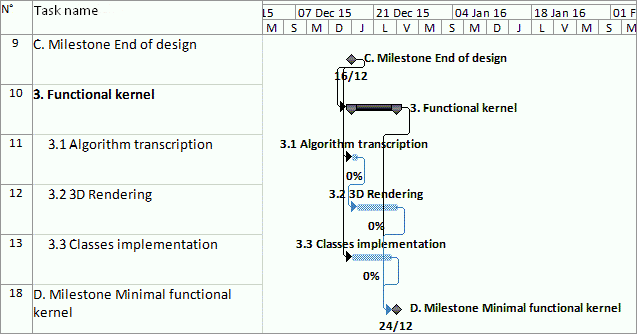
\includegraphics[height=3.7cm]{Images/Gantt_Reference_common.png}\\
			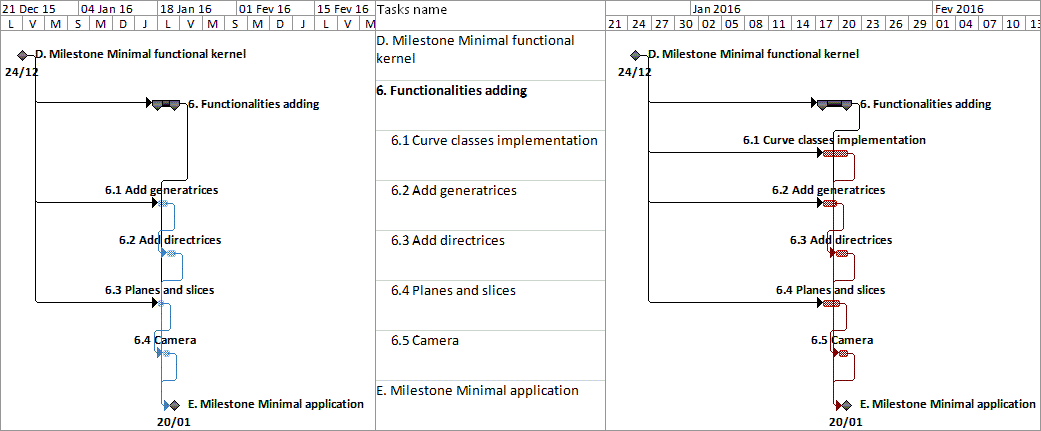
\includegraphics[height=4.3cm]{Images/Gantt_Comparaison.png}
		\end{center}
	\end{frame}


	\begin{frame}{\subsecname}
		\begin{center}
			\vspace{-0.2cm}
			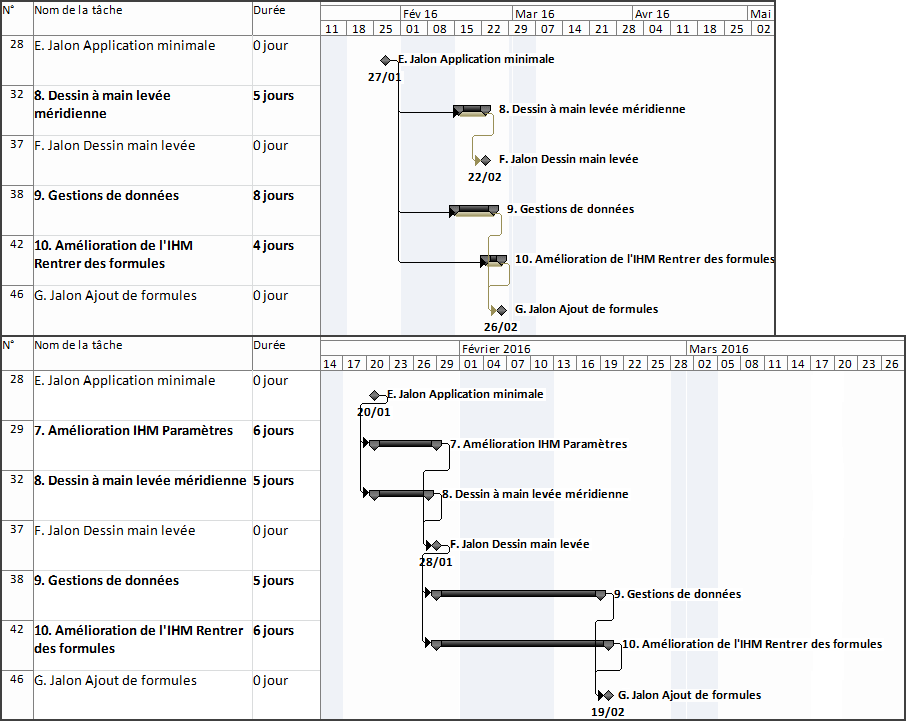
\includegraphics[height=8cm]{Images/Gantt_Diff.png}
		\end{center}
	\end{frame}


% --- Avancement ---------------------------------------------------------------
\subsection{Progress}
	\begin{frame}{\subsecname}
		\begin{figure}
			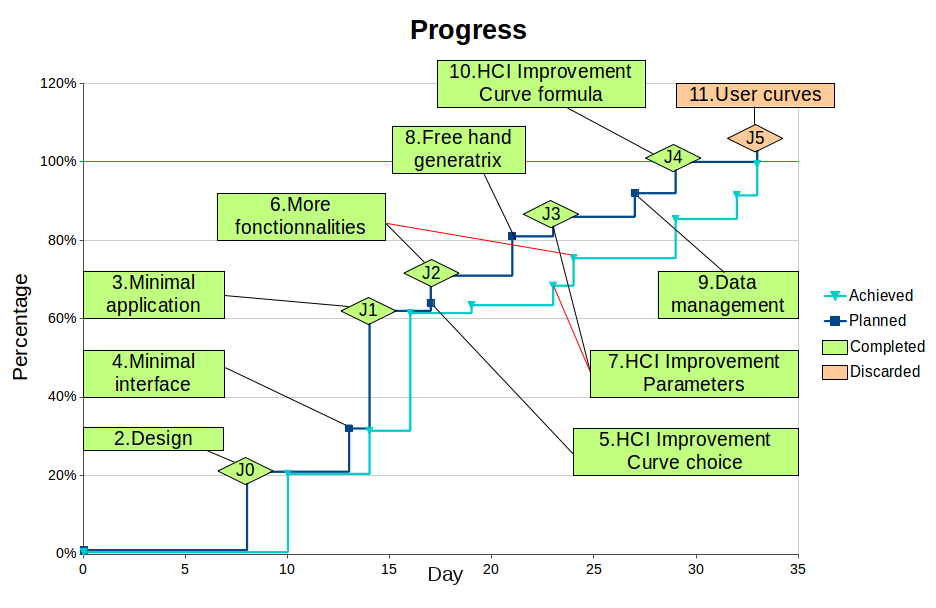
\includegraphics[width=12cm]{Images/avancement.png}
		\end{figure}
	\end{frame}


% --- Livrables ----------------------------------------------------------------
% barre un texte en rouge 50% (http://texdoc.net/texmf-dist/doc/generic/ulem/ulem.pdf)
\newcommand\Not{\bgroup\markoverwith{\textcolor{red!50!Black}{\rule[0.5ex]{2pt}{0.6pt}}}\ULon}

\subsection{Deliverables}
	\begin{frame}{\subsecname}
		\begin{center}
		{\renewcommand{\arraystretch}{1.2}
		\begin{tabular}{|c|m{4cm}<{\raggedright}|c|c|c|}
			\hline
			\textbf{\No} & \textbf{Deliverable} & \textbf{Tasks} & \textbf{Planned date} & \textbf{Actual date}\\
			\hline
			1 & Interface and \linebreak algorithm result & 2, 3, 4
				& Dec. 23{\small\textsuperscript{rd}} & Jan. 18{\small\textsuperscript{th}}\\
			\hline
			2 & Minimal application & 5, 6
				& Jan. 21{\small\textsuperscript{st}} & Jan. 25{\small\textsuperscript{th}}\\
			\hline
			2{\small\textsuperscript{bis}} & Multi-slice and \linebreak parameters & 7
				& --- & Jan. 29{\small\textsuperscript{th}}\\
			\hline
			3 & Free hand drawing and curves with editable \linebreak parameters & 7, 8
				& Jan. 29{\small\textsuperscript{th}} & Feb. 24{\small\textsuperscript{th}}\\
			\hline
			4 & Equations and export & 9, 10
				& Feb. 19{\small\textsuperscript{th}} & Feb. 24{\small\textsuperscript{th}}\\
			\hline
			5 & Final application \Not{and documentation} & 1 {\small to} 11
				& Mar. 2{\small\textsuperscript{nd}} & Mar. 2{\small\textsuperscript{nd}}\\
			\hline
			5{\small\textsuperscript{bis}} & Final documentation & 1
				& Mar. 11{\small\textsuperscript{th}} & Mar. 14{\small\textsuperscript{th}}\\
			\hline
		\end{tabular}}
		\end{center}
	\end{frame}



% --- Risk ---------------------------------------------------------------------
\subsection{Risks}
	\begin{frame}{List of risks}
		\begin{center}
		{\renewcommand{\arraystretch}{1.2}
		\begin{tabular}{|m{4.4cm}<{\raggedright}|c|c|c|l}
			\cline{1-4}
			\textbf{Risk} & \textbf{Gravity} & \textbf{Probability} & \textbf{Criticity} &\\
			\cline{1-4}
			Server linked problems & 1 & 0 & 0 & \Initial\\
			\cline{1-4}
			New clients & 1 & 2 & 1 & \Initial\Proven\\
			\cline{1-4}
			3D rendering needs too much ressources & 2 & 1 & 1 & \Initial\Proven\\
			\cline{1-4}
			Evolution of the generation \linebreak algorithm & 1 & 3 & 2 & \Initial\\
			\cline{1-4}
			Equipment/device dysfunction & 1 & 1 & 1 & \NewRisk\Proven\\
			\cline{1-4}
			Validation reveals serious technical problem & 2 & 1 & 1 & \Initial\\
			\cline{1-4}
		\end{tabular}}
		\end{center}
		\Initial\;Initial \hfill \NewRisk\;Added \hfill \Proven\;Encountered
	\end{frame}


	% Tableau risque
	\newcommand{\legendeRisque}{
		\small
		\begin{tabular}{|c|c|c|c|}
			\hline
			\textbf{Level} & \textbf{Gravity} & \textbf{Probability} & \textbf{Criticity} \\
			\hline
			\hline
			0 & None & < 1\% & \multirow{2}*{No critical}\\
			\cline{1-3}
			1 & Low & de 1\% à 5\% & \\
			\hline
			2 & Important & de 5\% à 20 \% & \multirow{2}*{Critical}\\
			\cline{1-3}
			3 & Dangerous & > 20\% & \\
			\hline
		\end{tabular}
	}



% --- Risk evolution -----------------------------------------------------------
	\begin{frame}{\subsecname}
		\begin{itemize}
			\item Server linked problems
		\end{itemize}
		\begin{figure}
			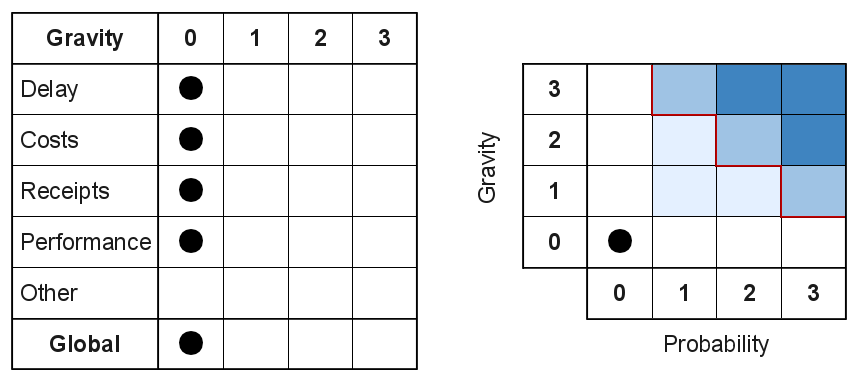
\includegraphics[width=8cm]{Images/risque_serveur.png}
		\end{figure}
		\begin{center}
			\legendeRisque
		\end{center}
	\end{frame}


	\begin{frame}{\subsecname}
		\begin{itemize}
			\item New clients {\color{white}p} % fix la position par raport à la diapo suivante/précédentes
		\end{itemize}
		\begin{figure}
			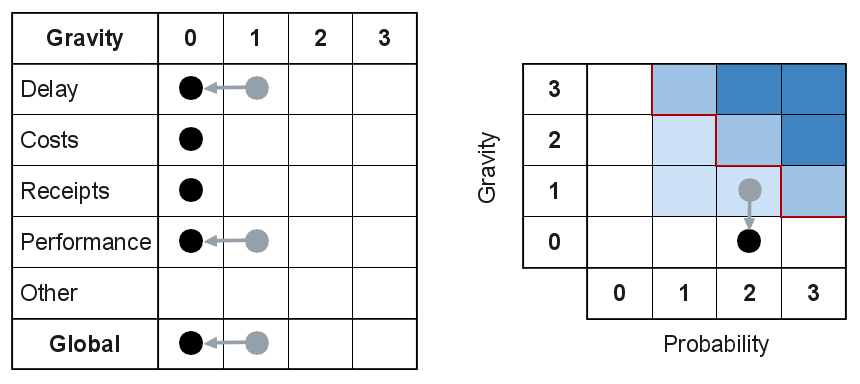
\includegraphics[width=8cm]{Images/risque_nouveau_client.png}
		\end{figure}
		\begin{center}
			\legendeRisque
		\end{center}
	\end{frame}
	
	
	\begin{frame}{\subsecname}
		\begin{itemize}
			\item Slow rendering
		\end{itemize}
		\begin{figure}
			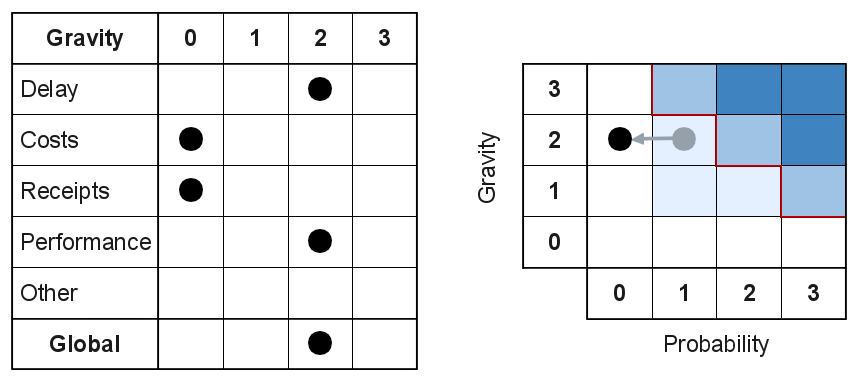
\includegraphics[width=8cm]{Images/risque_rendu.png}
		\end{figure}
		\begin{center}
			\legendeRisque
		\end{center}
	\end{frame}


	\begin{frame}{\subsecname}
		\begin{itemize}
			\item Evolution of the generation algorithm
		\end{itemize}
		\begin{figure}
			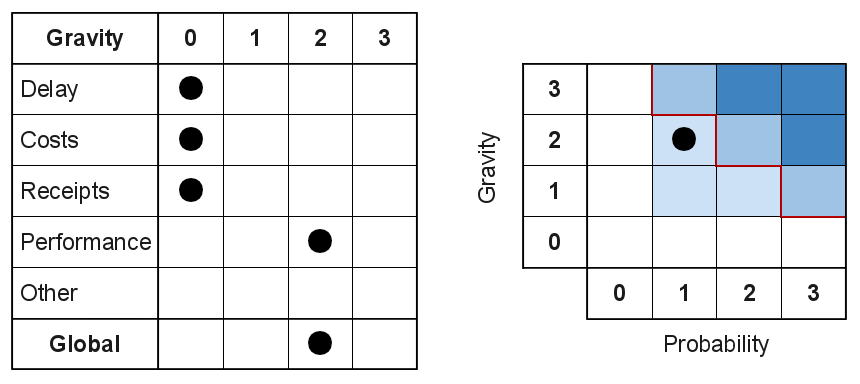
\includegraphics[width=8cm]{Images/risque_performance.png}
		\end{figure}
		\begin{center}
			\legendeRisque
		\end{center}
	\end{frame}	
	
	
% --- PAQL ---------------------------------------------------------------------
\subsection{Quality insurance plan}
	\begin{frame}{\subsecname}
		\begin{figure}
			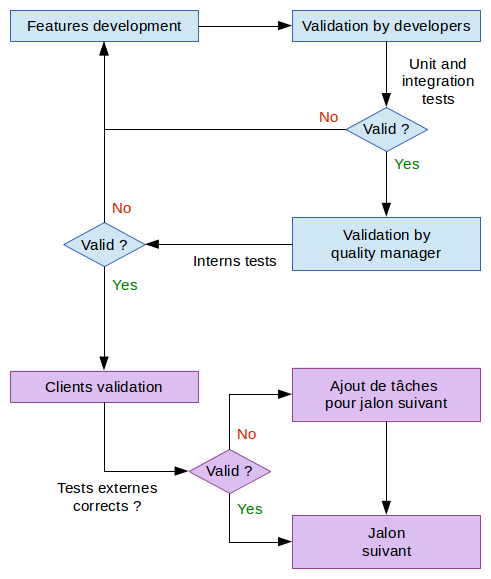
\includegraphics[height=7cm]{Images/PAQL_schema.png}
		\end{figure}
	\end{frame}


	\begin{frame}{ISO 9126}
		\begin{figure}
			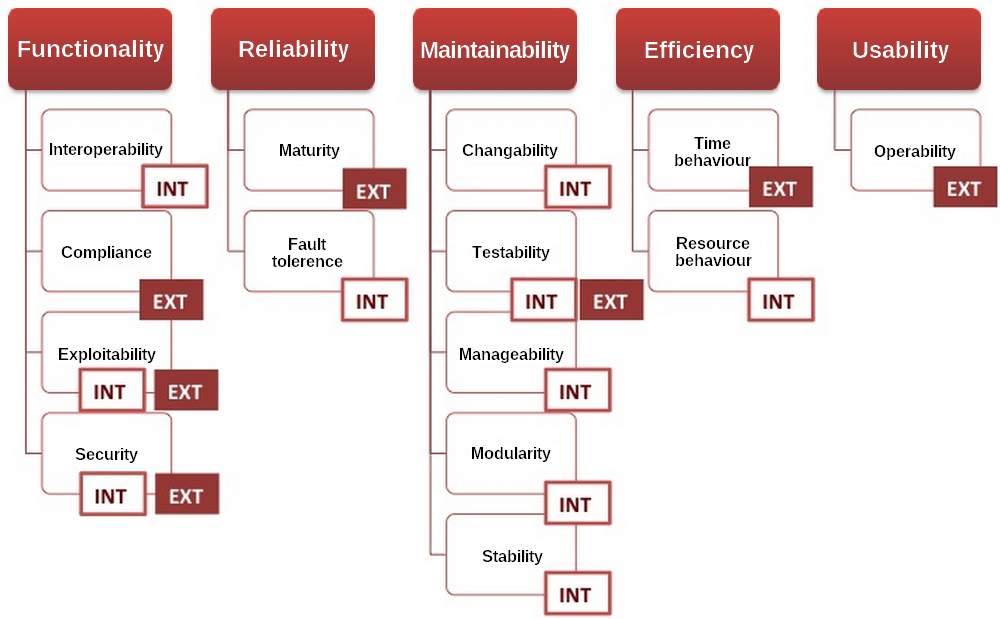
\includegraphics[height=7cm]{Images/iso9126.png}
		\end{figure}
	\end{frame}


	\begin{frame}{Software quality measurment}
		\begin{columns}
			\begin{column}{6cm}
				\begin{figure}
					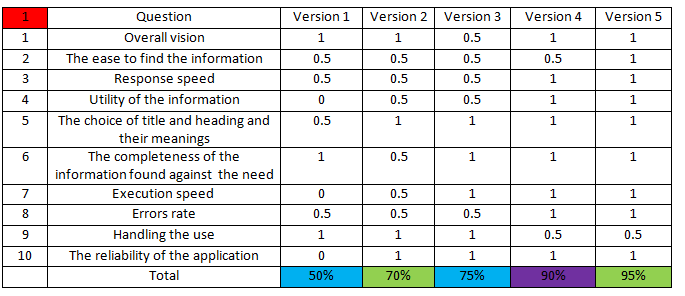
\includegraphics[width=6cm]{Images/ergonomie.png}
				\end{figure}
			\end{column}
			\begin{column}{7cm}
				\begin{figure}
					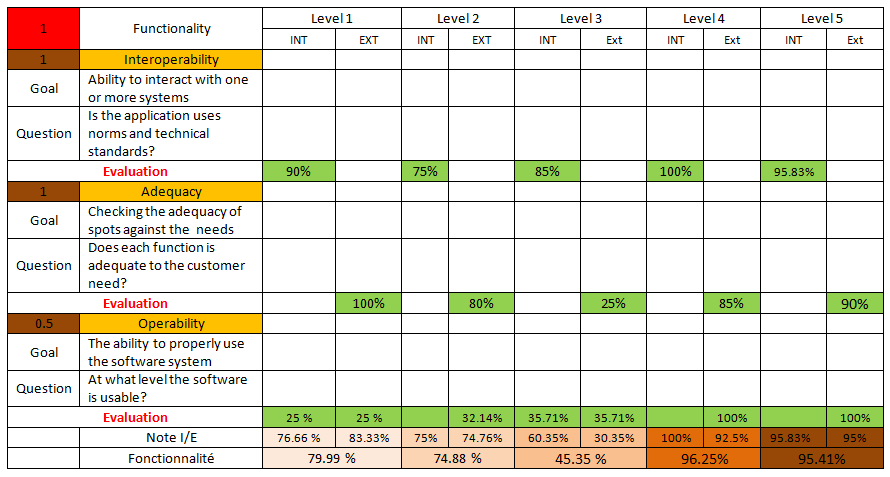
\includegraphics[width=6cm]{Images/fonctionality.png}
				\end{figure}
			\end{column}
		\end{columns}
	\end{frame}


	\begin{frame}{Software quality evaluation}
		\begin{figure}
			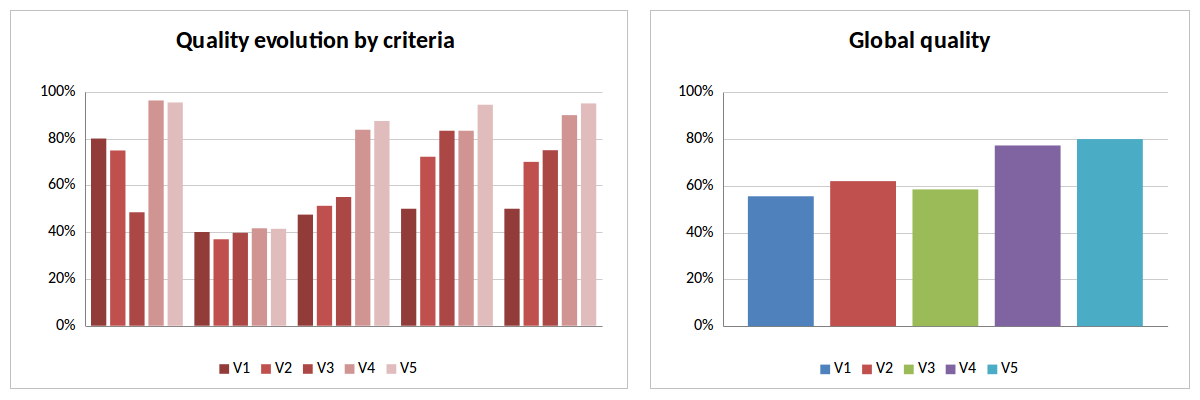
\includegraphics[width=12cm]{Images/resultat_qualite.png}
		\end{figure}
	\end{frame}


% --- Coût ---------------------------------------------------------------------
\subsection{Costs}
	\begin{frame}{\subsecname}
		\begin{figure}
			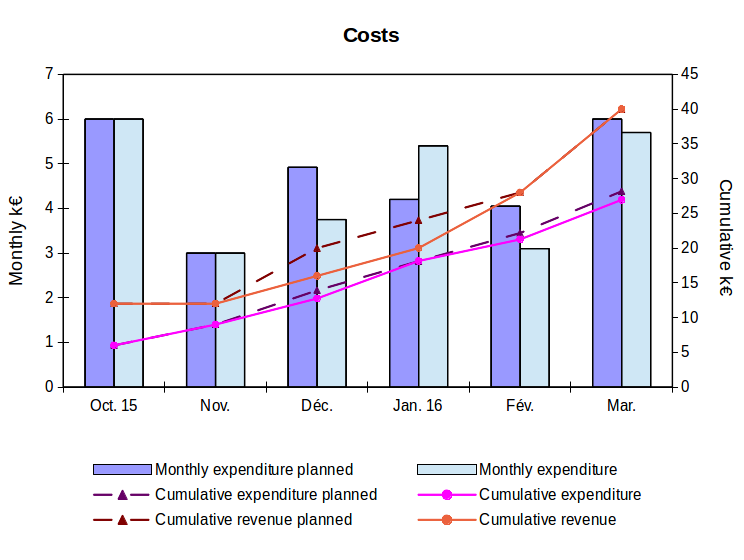
\includegraphics[height=7.5cm]{Images/cost2.png}
		\end{figure}
	\end{frame}



%===============================================================================
%	CONCLUSION
%===============================================================================


\section{Conclusion}


% --- Conclusion projet --------------------------------------------------------
\subsection{Technical aspect}
	\begin{frame}{\subsecname}
				\begin{itemize}
					\item Clients satisfied by the application
					\item Application available on \smallcaps{Xlim} website
					\item All main functionalities developed
					\item Final delivrable in two stage
					\item Possible improvements
					\begin{itemize}
						\item {\small{}X3D} export
						\item More information for users
						\item More types of curve
					\end{itemize}
					\item Perspectives
					\begin{itemize}
						\item New algorithms
						\item Lydie's internship subject
					\end{itemize}
				\end{itemize}
	\end{frame}


% --- Conclusion gestion projet ------------------------------------------------
\subsection{Project management aspect}
	\begin{frame}{\subsecname}
		\begin{itemize}
			\setlength\itemsep{1em}
			\item Weekly meetings with the pedagogic supervisor
			\item Interactions with clients
			\item Example of quality insurance plan
			\item Planning management
			\item Risks encountered
		\end{itemize}
	\end{frame}


% --- Conclusion perso ---------------------------------------------------------
\subsection{Personnal review}
	\begin{frame}{\subsecname}
		\begin{itemize}
			\setlength\itemsep{1.2em}
			\item Improvement in Javascript
			\begin{itemize}
				\item classes, inheritence, worker, etc.
				\item jQuery, MathJS, FileSaver
				\item WebGL
			\end{itemize}
			\item Spiral development: new experience
			\item Solving mathematical problem 
			\begin{itemize}
				\item base matrices
				\item drawing implicit curves
				\item etc.
			\end{itemize}
		\end{itemize}
	\end{frame}


% --- Remerciment --------------------------------------------------------------
\begin{frame}{}
	\bigskip
	\bigskip
	\begin{titleblock}{}
		\begin{center}
			\smallskip
			\Large Discrete 3D surfaces of revolution\\
			\medskip
			\small Final presentation
			\smallskip
		\end{center}
	\end{titleblock}

	\bigskip
	\begin{center}
		Thanks for your attention.\\
		\medskip
		Are there any questions\,?			
	\end{center}

	\bigskip
	\bigskip
	
\includegraphics[width=2cm]{../Images/logo-Xlim.png}
	\hfill
	
\includegraphics[width=2cm]{../Images/logo_univ_poitiers.png}
\end{frame}




\end{document}


